%Plantilla anteproyecto TFG
%Última modificación: 28 de mayo de 2021
\documentclass[twocolumn]{article}
%\usepackage[spanish]{babel}
\usepackage[utf8]{inputenc}
\usepackage{graphicx}
\usepackage{amsmath}
\usepackage{amssymb}
\usepackage{xcolor}
\usepackage{subfigure}
\usepackage{caption}
\usepackage{url}
%\usepackage{fancyhdr}
\usepackage[a4paper, margin=1in]{geometry}
\linespread{1}
\setlength{\parskip}{1\baselineskip}
\parindent 1cm
\sloppy

%Opciones que debes descomentar mientras estemos revisando el anteproyecto
%\usepackage{lineno}
%\linenumbers


\usepackage[pagebackref=true,breaklinks=true,letterpaper=true,colorlinks,bookmarks=true]{hyperref}
\usepackage{cleveref}  


%lista de palabras que Latex no parte bien
\hyphenation{mo-ne-ta-ry Fi-gu-re off-li-ne le-gi-ti-mate}

\begin{document}
%% Logo de la UAH
%\pagestyle{fancy}
%\fancyhead{}  % Limpia los encabezados
%\rhead{
\includegraphics[width=1cm]{Images/logo_UAH.png}}
%\setlength{\headsep}{1.5cm} 
%% Logo de la UAH
\thispagestyle{empty}
\onecolumn
\begin{center}

\begin{large}
Departamento de Física y Matemáticas\\
Escuela Politécnica Superior\\
\end{large}
\vspace{1cm}


\includegraphics[width=8cm]{Images/logo-uah.pdf}

\textbf{ANTEPROYECTO}

\vspace{1cm}

\begin{large}\textbf{\textit{Design, implementation and testing of a blockchain system to prevent fraud in the context of second-hand vehicle sales}}\end{large}

\vfill

February - 2025

\end{center}

\begin{flushright}
\textit{Autor - \textbf{Julio Álvarez Villaescusa}} \\
\textit{Director - \textbf{Héctor Ildecar Prieto Alfonso}}
\end{flushright}

\newpage
\twocolumn
\section{Introduction}
Fraud in the second-hand car market is a globally significant issue, with numerous scams occurring annually \cite{duboka2009second}. The present document proposes the utilization of emerging blockchain technologies for the purpose of preventing any fraud related second-hand vehicle sales.


\subsection{Blockchain's state of art}
The first reference to blockchain technology dates back to 1991 \cite{haber1991time}. However, the most prominent implementation of blockchain was introduced in 2008 by an individual using the pseudonym "Satoshi Nakamoto" \cite{nakamoto2008bitcoin}. Since then, numerous applications for this technology have emerged beyond the monetary system proposed in the original paper. These applications include:
\begin{itemize}
    \item Blockchain in financial management \cite{pal2021blockchain}
    \item Blockchain in security and privacy \cite{taylor2020systematic}
    \item Blockchain in IoT (see \cref{def:iot}) \cite{wang2019survey}
    \item Blockchain in transportation \cite{humayun2020emerging}
    \item Blockchain in healthcare \cite{agbo2019blockchain}
    \item Blockchain in education \cite{alammary2019blockchain}
\end{itemize}
\noindent The number of applications for blockchain technology has not only grown significantly, but also the volume of academic and industry articles discussing this technology has increased, as illustrated in Figure~\ref{fig:articles_per_y}. \cite{9786734}
\begin{figure}[h]
    \centering
    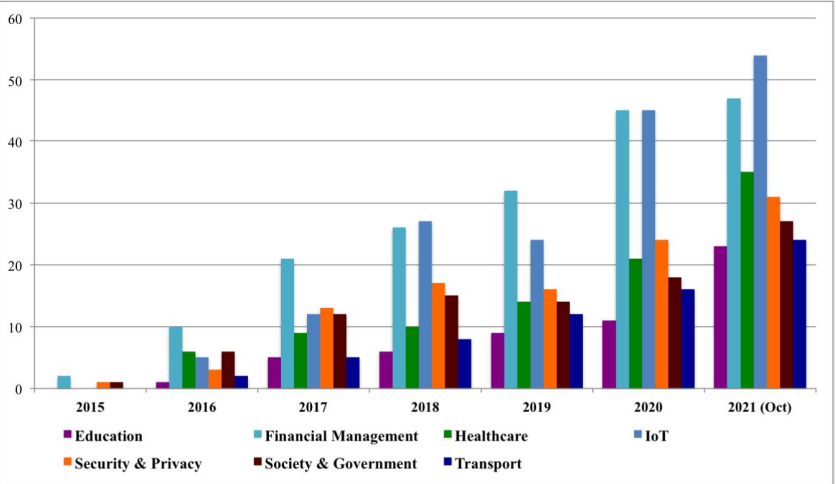
\includegraphics[width=1\linewidth]{Images/yearly_blockchain_articles.png}
    \caption{Blockchain articles per year}
    \label{fig:articles_per_y}
\end{figure}


\newpage
\section{Objectives and \\ application fields}
%Destaca los objetivos particulares, y también los campos de aplicación (haz una lista con las aplicaciones reales de tu trabajo).
The objective of this thesis is to develop a prototype of a blockchain solution that will facilitate the processing of vehicle history data in a secure and efficient manner, thereby ensuring effective data management.

\noindent The applications of this thesis are:
\begin{itemize}
    \item Mitigating the risk of fraud in second-hand car sales
    \item Preventing database compromise by distributing data through multiple nodes
    \item Streamlining bureaucratic processes through automated information management
    \item Consolidating disparate data types on a single ledger 
\end{itemize}

%All of this is a result of using a distributed transparent ledger to store car accidents, car transfers, and vehicle inspections.

\section{Work description}
%Ahora si, ¿cómo vas a hacer las cosas? Describe las partes, módulos o fases de tu proyecto, y añade un diagrama de bloques. Comenta cada uno de ellos, para que el lector entienda lo que persigues.
The preliminary phase of the process will entail the conceptualization of the blockchain, encompassing the determination of all its constituent elements and the formulation of a rationale for their inclusion. The aforementioned elements include:
\begin{itemize}
    \item Block header
    \item Block content
    \item Consensus mechanism
    \item Nodes (Actors)
    \item P2P type of network (see \cref{def:p2p})
    \item Transactions
    \item etc... \cite{patel2020review}
\end{itemize}

\noindent Once the design and functionality of the blockchain are defined, the implementation of the network deployment tool using Docker will commence. This tool will facilitate testing the blockchain and will include a corresponding testing phase to ensure its effectiveness.

\noindent Upon completion of the testing tool, the remaining aspects of the blockchain will be implemented, as previously discussed. Once the blockchain is complete, it will undergo intensive testing with the aforementioned tool.

\newpage


\section{Development phases}
%Ahora debes detallar, de forma técnica, las fases de desarrollo. Te pongo un ejemplo.
%\textcolor{red}{IMPORTANTE: debes indicar en cada item la duración de esa fase del proyecto}.
\begin{enumerate}
    \item \textbf{Bibliographic study of blockchain and distributed systems.} Duration: 3 weeks.
    \item \textbf{Blockchain designing.} Duration: 1 month.
    \item \textbf{Implementation of the blockchain's testing and deployment tool.} Duration: 1 month and 2 weeks. 
    \begin{itemize}
        \item Generation of docker images. Duration: 5 days.
        \item Image testing. Duration: 2 days.
        \item Deployment script implementation. Duration: 1 month.
        \item Tool testing and refining. Duration: 1 week.
    \end{itemize}
    
    \item \textbf{Implementation of the blockchain following the previous design.} Duration: 1 month. \begin{itemize}
        \item Consensus mechanism implementation. Duration: 1 week.
        \item Block implementation. Duration: 1 week.
        \item Node communications and role implementation. Duration: 2 weeks.
    \end{itemize}
    
    \item \textbf{Integrating the blockchain and the testing and deployment tool.} Duration: 1 week.
    \item \textbf{Code refactoring and documentation.} Duration: 1 week.
    \item \textbf{Thesis writing using \LaTeX.} Duration: 1 month.
\end{enumerate}

\begin{figure}[!h]
    \centering
    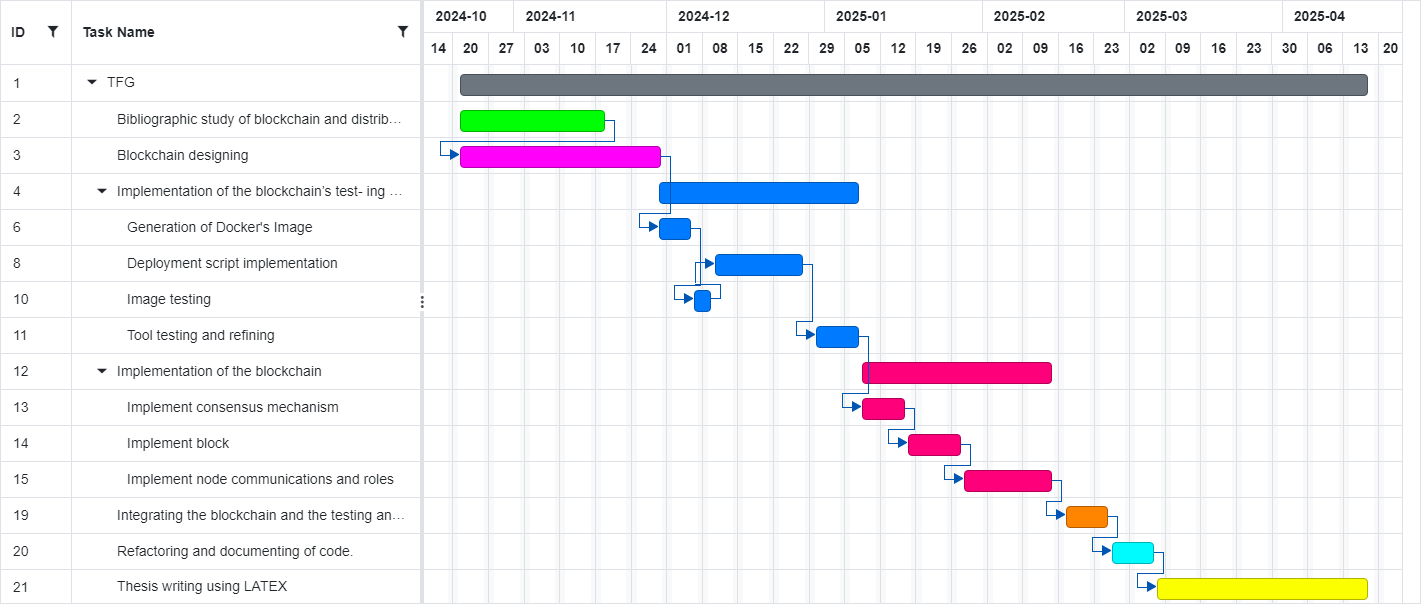
\includegraphics[width=2.2\linewidth]{Images/Grantt TFG.png}
    \captionsetup{justification=raggedright}
    \caption{Grantt Diagram of development phases}
    \label{fig:Grantt diagram}
\end{figure}

\newpage
\noindent A Grantt diagram representing the previously described phases can be seen in Figure~\ref{fig:Grantt diagram}.
%\newpage
\section{Resources}

%Describe los medios que vas a emplear para realizar el TFG: tipo de ordenador, software, SO, librerías, acceso a servidores de cálculo, plataformas robóticas concretas, bases de datos, etc.
The project will be developed using Python as the primary programming language. Additionally, the following technologies will be employed:
\begin{itemize}
    \item Docker (see \cref{def:docker})
    \item WSL (see \cref{def:wsl})
    \item socket libraries
    \item hashing libraries
    \item Git (see \cref{def:git})
\end{itemize}
Each of these technologies will be accompanied by their corresponding official documentation.

\noindent In this study, Visual Studio Code (VSCode) will be employed as the main code editor. To ensure adherence to best practices, linter extensions will be utilized. Additionally, a Docker extension will be leveraged to facilitate the management of container and images. Furthermore, Python debugging and highlighting tools will be incorporated to enhance the efficiency of the coding process.

\noindent The thesis will be written in \LaTeX\ (see \cref{def:latex}), utilizing Overleaf as the online editor and \TeX Studio as the offline editor.


\newpage
\section{Limitations}
\subsection{Scalability}
\vspace{-10pt}
The number of deployable nodes is limited by hardware constraints, hindering full scalability assessment of the blockchain.
\vspace{-20pt}

\subsection{Failure and Consistency Testing}
\vspace{-10pt}
Simulating node failures, slow networks \texttt{(e.g., 500ms $\le$ latency per node-to-node message)}, or partitions is limited, restricting the ability to test the blockchain’s reliability and consistency under adverse conditions.
\vspace{-20pt}

\subsection{Security}
\vspace{-10pt}
Running nodes locally may not accurately simulate external threats, making it difficult to perform security tests such as DoS attacks (See \cref{def:DoS})  or internal breaches.

\section{Definitions}

\label{def:iot}
\noindent\textbf{Internet of Things (IoT)} is the network of interconnected devices that collect and exchange data through the internet.


\label{def:p2p}
\noindent\textbf{Peer-to-Peer (P2P)} is a decentralized network model in which peers share resources directly without the need for a central server.

\label{def:docker}
\noindent \textbf{Docker} is an open-source platform for developing, deploying, and running applications in \textbf{containers}.


\label{def:wsl}
\noindent \textbf{WSL (Windows Subsystem for Linux)} is a compatibility layer that enables running a Linux distribution natively on Windows.


\label{def:git}
\noindent \textbf{Git} is a distributed version control system that tracks changes in source code, allowing for efficient management of project history and the ability to revert or merge modifications.




\label{def:latex}
\noindent \textbf{LaTeX} is a typesetting system used for creating scientific and technical documents, especially those with complex formulas and structured layouts.

\label{def:DoS}
\noindent \textbf{DoS (Denial of Service)} attack is a malicious attempt to overwhelm the resources of a system, service, or network, making it inaccessible to legitimate users by consuming its bandwidth, memory, or processing capacity.

\label{def:DoS}

\newpage
%Bibliografía
\bibliographystyle{unsrt}
\bibliography{bibliografia-tfc}


\end{document}
